\documentclass[11pt]{article}

\usepackage[a5paper,left=2cm,right=1cm,top=1cm, bottom=1.5cm]{geometry}
\usepackage{array}
\usepackage{makecell}
\usepackage[all]{nowidow}
\usepackage{wrapfig}
\usepackage{enumitem}
\usepackage{multicol}

\usepackage{hyperref}
\hypersetup{
    colorlinks=true,
    urlcolor=sokolblue,
    }

\usepackage[czech]{babel}
\usepackage[utf8]{inputenc} 
\usepackage{ellipsis}

\usepackage{fontspec}
\newfontfamily{\tyrs}{Sokol Tyrs}
\newfontfamily{\fugner}{Sokol Fugner}

% \usepackage{lmodern}
% \usepackage[T1]{fontenc} 
\usepackage{anyfontsize}
\newcommand{\titlesize}{\fontsize{56pt}{67pt}}


\usepackage[dvipsnames]{xcolor}
\definecolor{sokolred}{RGB}{228, 5, 33}
\definecolor{sokoldarkred}{RGB}{200, 0, 30}
\definecolor{sokolblue}{RGB}{45, 46, 135}

\usepackage{tikz}
\usetikzlibrary{calc}

\usepackage{fancyhdr}

\fancypagestyle{standard}{%
    \fancyhf{}
    \fancyhead[LO]{%
        \begin{tikzpicture}[overlay,remember picture]
            \fill [color=sokolred] (current page.north west) rectangle ($ (current page.south west) + (1cm,0cm) $);
            \fill [color=sokolred] ($ (current page.north west) + (1.1cm,0cm) $) rectangle ($ (current page.south west) + (1.2cm,0cm) $);
        \end{tikzpicture}
        }
    % \fancyhead[RE]{%
    %     \begin{tikzpicture}[overlay,remember picture]
    %         \fill [color=orange](current page.north east) rectangle
    %             ($ (current page.south east) + (-1cm,0cm) $);
    %     \end{tikzpicture}
    %     }
    \fancyfoot[C]{%
      \begin{tikzpicture}[overlay,remember picture]
        \fill [color=sokolred] ($ (current page.south east) + (-1.5cm,1.3cm) $) rectangle ($ (current page.south east) + (0cm,0.5cm) $)
         node [pos=0.5,color=white] {\large\tyrs{\thepage}\hspace*{0.5cm}};
      \end{tikzpicture}
    }

    \renewcommand{\headrulewidth}{0pt}
    \renewcommand{\footrulewidth}{0pt}
}



\fancypagestyle{uvodnik}{%
    \fancyhf{}
    \fancyfoot[C]{%
      \begin{tikzpicture}[overlay,remember picture]
        \fill [color=sokolred] ($ (current page.south east) + (-1.5cm,1.3cm) $) rectangle ($ (current page.south east) + (0cm,0.5cm) $)
         node [pos=0.5,color=white] {\large\tyrs{\thepage}\hspace*{0.5cm}};
      \end{tikzpicture}
    }

    \renewcommand{\headrulewidth}{0pt}
    \renewcommand{\footrulewidth}{0pt}
}

\fancypagestyle{blank}{%
    \fancyhf{}
    \fancyfoot[C]{}

    \renewcommand{\headrulewidth}{0pt}
    \renewcommand{\footrulewidth}{0pt}
}


\newcommand{\post}[1]{%
\begin{center}
{\huge \tyrs #1}
\end{center}
}

\newcommand{\subpost}[1]{%
\vspace*{12pt}
\begin{center}
{\Large \tyrs #1}
\end{center}}

\newcommand{\signature}[2]{%
  \begin{flushright}
    \textbf{#1}\\#2
  \end{flushright}
}

\newcommand{\luv}{\clqq\kern-0.07em}
\newcommand{\ruv}{\kern0.07em\crqq\kern0.1em}

\usepackage{csquotes}
\DeclareQuoteAlias{german}{czech}
\MakeOuterQuote{"}

\usepackage[normalem]{ulem}


\begin{document}

%% title
\newgeometry{margin=1cm}
\pagecolor{sokolred}
\color{white}
\pagenumbering{gobble}
\begin{center}
\vspace*{\fill}

{\titlesize \fugner ZPRÁVY}

{\titlesize \tyrs SOKOLA LIBEŇ}

\vspace*{1cm}

{\large ročník XLIX · číslo 4 · listopad 2023}

\vspace*{\fill}
\end{center}

\clearpage
\normalcolor
\nopagecolor
\pagenumbering{arabic}

%% úvodník
\pagestyle{uvodnik}
\newgeometry{margin=1.5cm}


{\fontsize{48pt}{57pt} \fugner \color{sokolred} \noindent Úvodník}

\vspace*{12pt}

\noindent
Vážení členové Sokola Libeň,

\noindent
v~Sokole se toho stále děje mnoho, přesto nyní probíhá něco, co bych chtěl vyzdvihnout.

Jak jste jistě zaznamenali, v~sokolovně probíhá rozsáhlá rekonstrukce šaten. Ač to na první pohled nemusí být patrné (vždyť jsou to “jenom” šatny), jde o~nejrozsáhlejší rekonstrukci v~sokolovně za posledních 20 let. Tehdy byla provedena celková oprava fasády a opravy střech, které byly z~velké části financovány z~prodeje penzionu Sokolí boudy v~centru Dolní Malé Úpy v~Krkonoších, který byl ve vlastnictví jednoty. Bohužel na rekonstrukci vnitřních prostor sokolovny již prostředky nevystačily. V~posledních 20 letech tak byly prováděny spíše jen dílčí opravy. 

O~potřebě rekonstrukce interiéru sokolovny se hovoří již řadu let, přičemž situace šaten byla dlouhodobě nejméně utěšená. Samotné přípravy na rekonstrukci šaten zabraly přibližně 10 let –⁠ od prvních studií, jak by šatny měly vypadat, přes projektovou dokumentaci, získání stavebního povolení, získání finančních prostředků až po výběr dodavatele a samotné zahájení stavebních prací. To vše je navíc komplikováno skutečností, že budova sokolovny je kulturní památkou, což přináší řadu omezení, delší dobu přípravy i vyšší náklady.

Nakonec se vše úspěšně podařilo, rekonstrukce probíhá a snad se již pomalu blíží ke svému cíli, byť k~jeho dosažení nás čeká ještě spousta práce, a to jak částečně na samotné stavbě, tak zejména na zajištění kolaudace a možnosti tím pádem šatny řádně užívat. 

Rekonstrukce přináší řadu obtíží, které stavbu provází, za což se chci všem členům omluvit. Věřím však, že se rekonstrukci podaří co nejdříve řádně dokončit a nové šatny včetně souvisejícího zázemí zvýší komfort všem uživatelům sokolovny. Tímto však práce na sokolovně zdaleka nekončí. Ač se jedná o~nejrozsáhlejší rekonstrukci za poslední dekády, je to jen zlomek toho, co je potřeba na sokolovně opravit. Obnova sokolovny je nekonečný příběh.

\signature{Jan Přibyl}{člen výboru a cvičitel žáků}

\clearpage

%% termínka

\pagecolor{sokolred}
\color{white}
\renewcommand{\arraystretch}{1.4}

\newcommand{\boxheight}{13.5cm}

\vspace*{\fill}
\post{TERMÍNOVÁ LISTINA AKCÍ JEDNOTY}
\vspace*{0pt}

\begin{center}
\begin{tikzpicture}
  \draw [ultra thick,color=white](0.3cm,0cm) rectangle (12.3cm,\boxheight);
  \fill [color=white] (0cm,0.3cm) rectangle (12cm,\boxheight + 0.3cm)
  node [pos=.5, color=black] {
    \begin{tabular}{l  p{6.5cm}}
      30. 11. 2023 (čt) & Mikuláš \\
      16. 12. 2023 (so) & Rychlý šplhoun v~Sokole Kobylisy \\
      20. a 21. 12. 2023 (st, čt) & Vánoční nadílky turisťáků \\
      21. 12. 2022 (čt) & Loutkáři (vánoční loutkové představení) a poslední cvičení v~roce 2022 \\
      5. 1. 2024 (pá) & Silvestr cvičitelů \\
      10. 2. 2024 (so) & Memoriál Jana Vorla \\
      20.+22. 2. 2024 (út, čt) & Nominační závody žáků \\
      2. 3. 2024 (so) & Akademie (přesunutá z~podzimu) \\
      3. 3. 2024 (ne) & Brigáda jaro \\
      20. 3. 2024 (st) & Valná hromada \\
      23. 3. 2024 (so) & Dětské a Dospělácké Šibřinky \\
      13. 4. 2024 (so) & 66. Jarní Výlet Libeňského Sokola \\
      25.-26. 5. 2024 & Oblastní Slet v~Brandýse nad Labem \\
      30. 5. 2024 & Dětský den \\
      15. 6. 2024 & Oblastní slet ve Voticích \\
      30. 6. 2024 & Sletový průvod Prahou \\
      4. 7. 2024 & Program sletových skladeb I. (Eden) \\
      5. 7. 2024 & Program sletových skladeb II. (Eden) \\
      5. 7. 2024 & Posletový táborák \\
    \end{tabular}
  };
  %  node [color=black] {FOOBAR};
\end{tikzpicture}

\renewcommand{\arraystretch}{1}

\vspace*{12pt}
Sledujte naše stránky a zprávy ze systému EOS, kde budeme postupně uveřejňovat podrobnosti k~jednotlivým akcím.

\end{center}
\vspace*{\fill}

\clearpage
\nopagecolor
\normalcolor

%% normální obsah
\restoregeometry
\pagestyle{standard}

\post{Rekonstrukce šaten\\\Large{(a další stavební akce)} }
Jak si jistě pamatujete, před létem jsme obdrželi šestimilionový grant od Magistrátu hl. m. Prahy na rekonstrukci šaten s~podmínkou dokončení do konce tohoto roku.

Rekonstrukce šaten zatím pokračuje takřka podle plánu (zpoždění oproti harmonogramu je asi 3 týdny), ale měla by skončit opravdu do konce tohoto roku. Smlouva na grant byla podepsána 20. června, 19. července jsme měli definitivně vybranou firmu z~veřejné zakázky (uběhly všechny zákonné lhůty), podepsali jsme smlouvu, předali staveniště a ještě ten den začala firma Wandel s~pracemi. Od té doby je firma na stavbě každý všední den a většinou i soboty. Podlaha byla vykutána, nová včetně podlahového topení vybetonována. Jsou hotové nové příčky ve sprchách (mají úplně novou dispozici) a též je tam podlahové vytápění a beton. Jsou hotovy veškeré rozvody vody, odpadů a elektřiny a dokončuje se topení. Nyní se začínají štukovat stěny, příští týden nastoupí obkladači do sprch. Lakýrník si má vzít do parády dveře. Následně se vymaluje, udělá se epoxidová podlaha, nainstaluje se vzduchotechnika, která už leží připravená ve skladu, připravené šatní kóje, skříňky, osvětlení, udělá se teraco podlaha v~předšatní a namontují se (již hotové) botníky. Pak ještě udělat sádrokartonové podhledy na WC a ve sprchách, namontovat umyvadla, WC mísy a sprchové hlavice a máme hotovo. Tak doufejme, že to množství zbývající práce firma stihne. Po Novém roce nás čeká ještě úředničina s~kolaudací (a případným užíváním před kolaudací) a budeme se moci těšit z~nových šaten. Do té doby se omlouváme za prach, hluk, provizorní šatny a další ústrky, ale bez toho bychom se k~novým šatnám nikdy nedostali. Kromě prací dle projektu jsme přiobjednali i kompletní revitalizaci zadních schodišť, abychom to měli až do sálu celé nové.

S~novými šatnami přijdou i změny v~režimu jejich používání. Tou nejzásadnější bude to, že v~prostoru před šatnami budou umístěny botníky, kde si každý odloží své venkovní boty, a do šaten se už bude vstupovat v~sálové obuvi nebo bos. Další změnou bude používání šatnových kójí (pro větší oddíly jako doposud) a skříněk (malé oddíly a jednotlivci), ke kterým se budou půjčovat zámečky, přičemž pokaždé budete mít jinou skříňku. Část skříněk půjde i pronajmout na pololetí či cvičební rok, jako to bývalo. Podrobnosti sdělíme ještě před otevřením šaten.

Za šatny zaplatíme 10 500 000 Kč vč. DPH (z~grantu máme 5 997 000 Kč). I~po zaplacení by nám na účtu jednoty mělo zbýt cca 500 000 Kč. Není to moc, ale zatím to vypadá, že to finančně zvládneme bez nutnosti půjčky.
Kromě šaten nás příští rok čeká propojení místnosti bývalé matriky s~nájemcem ABA strategie, který má zájem o~prostor opuštěný firmou Direkta. Připravujeme projekt (památkáři, statika a stavební povolení) a smlouvu o~smlouvě budoucí s~novým nájemcem, abychom to mohli během jara zrealizovat a cca od července pronajmout. 

Po dodání stanoviska od památkářů podáme žádost o~kolaudaci podzemní místnosti (nové loděnice), která je hotová.

Byla opravena římsa nad vchodem do župy a komínový štít a čeká nás oprava malé severní terasy, kterou zatéká do místnosti nájemce Netsystem.

Také jsme podepsali rezervační smlouvu na nákup louky nedaleko Trhových Svin pro tábory našich turistických oddílů a začínáme s~přípravami akcí ke 140. výročí vzniku naší jednoty (1884), které nás čeká příští rok na podzim. 

\signature{Jiří Novák (Jirkan)}{starosta\\tel.: 602 284 198}

\vspace*{24pt}

\post{Zpráva místonáčelníka}
\vspace*{-12pt}
\subpost{Podzim (nejen) v~oddíle žáků a dorostenců}
Ml. žáci (2014–⁠2017) cvičí v~út a čt v~17–18, st. žáci a dorostenci (2006–⁠2013) v~út a čt v~18–19. Pro cvičitele a dorostence možnost úterního cvičení mužů a čtvrteční košíkové (oboje 19–20).

Cvičení venku (park, zahrada sokolovny) s~atletickými disciplínami začalo po prázdninách a za neuvěřitelně příznivého počasí trvalo do 5. řijna. Dvakrát jsme posloužili studentům FTVS jako studijní materiál k~jejich studiu – dívali se, jak to v~praxi taky může vypadat. Od 10.~října cvičíme už jen v~sokolovně – kromě gymnastiky nezapomínáme na rozcvičku a hry.

Také jsme postupně začali nacvičovat se staršími a posléze i s~mladšími žáky na slet. Od 14. 11. jsme nácvik rozjeli naplno, neboť dorazilo sletové náčiní. Zatím máme přihlášeno 27 mladších žáků (původně jsme počítali s~16, už jsme navýšili na 24 a možná dáme s~dopomocí jednoty na Proseku i 32). Starších je zatím 24, tedy tolik, kolik jsme počítali. 

V~tuto chvíli je už spuštěna i jednoduchá \textit{Zimní soutěž – Shyby} (s~variantou pro ty, kteří nezvládnou – výdrž ve shybu, kam budou vysazeni). 

Nakonec do hodin ještě před koncem roku vměstnáme i nácvik na březnovou akademii a únorové nominační závody v~gymnastice. Bude to složité, ale vše musíme stihnout.

Pevně věříme, že kluci i díky Vám přivedou další nové kamarády – stále máme místo pro další zájemce o~cvičení, které rádi uvítáme (bereme mladší i starší žáky).

V~loňském cvičebním roce jsme měli zapsáno 127 cvičenců (66 mladších žáků, 32 starších žáků, 13 dorostenců a 16 cvičitelů) a průměrná docházka na hodinu byla 52,53 při měsíčním průměru zapsaných 100,7. Letos je zatím zapsáno 127 cvičenců (59 mladších žáků, 38 starších žáků, 13 dorostenců a 17 cvičitelů) a průměrná docházka na hodinu byla v~září 60,71 a v~říjnu 62,63.
V~tuto chvíli se počítají výsledky letních disciplín (vyhlášení proběhne začátkem roku 2024). Trvá také celoroční soutěž \textit{O~nejvěrnější docházku} s~pravidelným každoměsíčním vyhlašováním a rozdáváním diplomků za 100\% docházku.

Děkujeme za vzorné zaplacení příspěvků na druhé pololetí roku 2023.
O~kluky se stará náš mužský cvičitelský sbor ve složení: cvičitelé: J. Novák (53), T. Novák (51), J. Kudroň (35), J. Přibyl (32), J. Kubišta (31), J. Kerhart (21), P. Boháč (20), a naši mladí pomahatelé: J. Skokan, T. Kléger, V. Novák, V. Blahunek, J. Pikálek a A. Basseville. 

\subpost{Nabídka dalších oddílů}
Všem žákům nabízíme možnost účasti na výletech, které pořádají naše \textbf{turistické oddíly}. Káňata zvou mladší žáky, Jilm a Veverky žáky starší. Mladší děvčata mohou chodit též do Káňat, starší do Jilmu a Veverek. Všechny oddíly též samozřejmě nabízejí i členství – což znamená středeční (Jilm a Veverky) či čtvrteční (Káňata) schůzky v~klubovně a výpravy, které se konají cca \(1\times\) měsíčně. Vyvrcholením celoroční činnosti je pak letní tábor. V~roce 2024 to bude opět Tajanov u~Velhartic na Šumavě. Informace u~vedoucích oddílů – viz informace u~oddílů na našich stránkách. 

Líbí se vám \textbf{cvičení mužů} na akademiích? Klidně se můžete stát členem oddílu – berou další zájemce (muže 18–50 let). Cvičí se v~úterý v~19–20. 

Výborně funguje před několika lety založený \textbf{oddíl šplhu} (osmimetrové lano ze sedu bez přírazu). Řada jeho členů se účastní i mistrovství republiky v~tomto sportu. Též berou další zájemce od staršího žactva až po muže a od loňska šplhají i děvčata a ženy. Další větví v~mnohotvárné činnosti mužů je \textbf{přetah lanem} – i v~tomto sportu se závodí a konají se i mezinárodní turnaje.

\subpost{Organizační informace}
\textbf{Pro zajištění hladkého nácviku na Slet prosíme rodiče, aby posílali kluky do Sokola, co to půjde, ať můžeme nacvičovat v~plném počtu} – je tam dost pohybu a spolupráce mezi cvičenci. Takže i ti, co mají zaplacenu jednu hodinu týdně, mohou chodit z~důvodu nácviku dvakrát týdně.

Děkujeme za používání matričního systému EOS. Platby příspěvků se nám tak letošní podzim sešly během několika málo dní. Na druhou stranu vás tímto kanálem dokážeme rychle a v~případě potřeby i cíleně informovat o~našich akcích. A~navíc, pokud vy potřebujete něco změnit, máte tak šanci to učinit sami (změna kontaktních údajů, zdravotního stavu apod.), případně lze změnit i oddíl či četnost hodin, a to tak, že se přihlásíte do systému, dáte „Nový požadavek na management“ a napíšete, co potřebujete. Kancelář to učiní a dá vám vědět, že se tak stalo.

V~matrice – 1. patro sokolovny (čtvrtek 15:45–18:45) lze pak zakoupit bílé tričko se znakem nebo znak na vlastní bílé tričko pro žáky.

\subpost{Akce jednoty mimo cvičení}
\textbf{Běh strmý} --- Ve čtvrtek 21. září se konal 23. ročník Běhu strmého do Zámeckého vrchu. Trať měří 199 metrů s~převýšením 29 metrů v~libeňském parku. Dorazilo rekordních 204 závodníků ve všech vypsaných kategoriích. Nejvyšším počtem závodníků se mohla pochlubit kategorie mladších žáků – bylo jich 41. Krátce po doběhu posledního závodníka začalo vyhlašování vítězů. Absolutním vítězem se stal časem 38,6\,s V. Paleta. Všichni si odnesli pamětní lísteček a drobnou sladkost. Kromě vlastního běhu proběhla i Sletová štafeta, kdy se na padesátimetrovém okruhu vystřídalo 206 běžců (někteří vícekrát) a uběhli tak štafetou 10 300 metrů. Kolem byly rozmístěny vývěsky s~fotografiemi a informacemi o~minulých sletech a pod vrbou se na plátno promítaly skladby připravované na blížící se slet v~roce 2024. Děkujeme všem 23 pořadatelům.

Cvičitelé (21) se po Běhu strmém sešli na pracovní schůzce, kde si rozdělili pořadatelství akcí, nácviky sletových skladeb a další úkoly, a také jsme určili data všech akcí až do června 2024.

\vspace*{12pt}
\noindent
\textbf{Památný den sokolstva} --- Ve čtvrtek 5. října proběhl pietní akt k~Památnému dni sokolstva. U~pamětní desky v~sokolovně byly položeny květiny a náčelník Josef Kubišta a Bára Jeníková a Martin Kubů ze vzdělavatelského odboru přednesli proslovy. Následoval přesun průvodem k~Rokytce a vypuštění asi 50 lodiček se svíčkami na památku sokolských obětí nacistické okupace.

\vspace*{12pt}
\noindent
\textbf{PVLS} --- Podzimní Výlet Libeňského Sokola (již 65. v~pořadí) a hlavně Sraz v~přírodě pražských žup proběhl v~sobotu 7. října. Ze 119 přítomných bylo (tradičně) 88 z~Libně (48 z~našich turistických oddílů Jilm a Veverky a Káňata a 40 dalších cvičenců, rodičů a hostů). Jelo se vlakem z~hlavního nádraží do Čtyřkol. Sešli jsme k~Sázavě a na jezu se zájemci mohli vykoupat v~řece, která měla teplotu 13 °C, a obdrželi tak Modrou stuhu (bylo to 35 lidí). V~tu chvíli se k~nám připojili i Jilmáci a Veverky na kolech, kteří měli tento víkend kolovku. Vystoupali jsme po modré značce ke kostelíku ve Lštění, kde byl zahajovací nástup srazu s~vyhlášením Pamatovačky, Jazykohrátek a Vaření. Kromě Libně bylo na výletě i 18 účastníků z~Jednoty Sokol Staré Město a 13 ze Sokola Zlíchov. Po nástupu jsme vyrazili směrem ke zřícenině Stará Dubá. Cestou jsme si v~lese zahráli několik kol běhací a chytací hříčky. Po příchodu na zříceninu byl oběd, vaření a volná zábava. Okolo třetí byl zakončovací nástup s~vyhlášením soutěží, Písnička, rozdání Pamětních lístečků a ukončení srazu. Libeňáci si ještě postavili kamenné věžičky a zahráli hříčku Salaoba. Pak už jsme se sebrali a vraceli se stejnou cestou k~vlaku. Na louce u~kostelíka ve Lštění jsme si ještě stačili zahrát 4 hříčky - Prodej roh, Na bouchanec, Na Titora a Lagori. Jarní výlet je naplánován na sobotu 13. dubna 2024.

\vspace*{12pt}
\noindent
\textbf{Listopadové střípky} --- V~pátek 10. 11. proběhla tradiční \textbf{plavecká štafeta O~pohár starostů pražských žup}. Naše župa obsadila v~dětské i dospělé kategorii 2. místo mezi třemi pražskými župami. Za Libeň závodil v~dospělácích muž L. Šimek. 

V~sobotu 11. 11. měli Jilmáci a Veverky již 43. ročník \textbf{hry Vyzvědači}. Tři skupiny navzájem zjišťují na území protivníka potřebné věci a sami tomu na svém území brání. Hrálo 25 dětí a 5 vedoucích.

V~sobotu 11. 11. proběhla také \textbf{Podzimní brigáda}. K~práci se sešlo 15 lidí (7 cvičitelů, 2 cvičitelky, 3 žáci, 1 žena a 2 muži), kteří se po rozdělení prací postarali o~posekání veškerých travnatých ploch, zametení listí na chodníku kolem sokolovny, zazimování doskočiště, opravu propadlé zámkové dlažby, opravu dveří do sálu, nátěr spár luxferů v~kanceláři, opravu krytů topení v~sále, umytí všech míčů, florbalových mantinelů a přeskokového náčiní, svaření prasklé konstrukce basketbalového koše, opravu florbalek a sítí florbalových branek, podlepení kopyt všech koňů, koz a beden filcem, aby neškrábaly parkety, úpravu závěsu, přendání bradel do druhé lodi, vyrobení nových závěsů na malé trampolínky a celkový úklid nářaďovny včetně přerovnání náčiní ve skříních. Pracovali jsme od 9 ráno do půl třetí odpoledne.

V~neděli 12. 11. \textbf{brigádnickou prací pokračovaly turistické oddíly}. Sešlo se 17 dětí a 4 vedoucí a od 9 do půl druhé stihli úklid klubovny a táborového vybavení v~dílně, opravu táborového nářadí, umytí žíněnek a cvičebních podložek v~sále, vyznačení míst pro značky na nácvik sletu v~sále, vytření sálu a zadních schodišť, přilepení lišty v~přízemí, opravu krabic na židle a odnos asi poloviny skládacích židlí na balustrádu.
Účastníkům děkujeme. 

\textbf{Výsledky závodů, fota, dopisy a další informace} najdete jednak na vývěskách v~sokolovně a na ní a také na www.sokol-liben.cz.

\subpost{A~co nás čeká ve cvičení v~nejbližších\\dnech a měsících: Plánované akce}
\textbf{Mikuláš} přijde do naší sokolovny ve čtvrtek 30. listopadu spolu s~čerty, anděly a punčochami pro hodné (a přihlášené) děti.

V~sobotu 16. 12. pořádá Sokol Kobylisy soutěž \textbf{Rychlý šplhoun}. Zájemci, hlaste se u~náčelníka.

Ve středu 20. 12. bude mít \textbf{vánoční nadílku} oddíl Jilm a Veverky a ve čtvrtek 21. 12. pak Káňata.

Ve čtvrtek 21. 12. od 17 hodin sehraje \textbf{loutkové divadlo libeňského Sokola Nástup vánoční představení}. Přijďte se podívat.

Poslední cvičení v~roce 2023 bude ve čtvrtek 21. 12., po Novém roce se sejdeme ve čtvrtek 4. ledna 2024.

Dále nás na jaře 2024 čekají tyto akce:
\begin{itemize}[
  itemsep=-3pt,
  leftmargin=2.5em,
  itemindent=-1em
]
  \item[] 5. 1. 2024 (pá) – \textbf{Silvestr cvičitelů}
  \item[] 10. 2. 2024 (so) – \textbf{Memoriál Jana Vorla}  – gymnastické závody pro dorostence a muže
  \item[] 20.+22. 2. 2024 (út, čt) – \textbf{Nominační závody žáků} – nominační závody pro žáky (výběr borců pro dubnové závody všestrannosti)
  \item[] 2. 3. 2024 (so) – \textbf{Akademie} (přesunutá kvůli rekonstrukci šaten z~tradičního listopadového termínu)
  \item[] 3. 3. 2024 (ne) – \textbf{jarní brigáda}
  \item[] 23. 3. 2024 (so) – odpoledne \textbf{Dětské šibřinky}, večer \textbf{Šibřinky pro dospělé}
\end{itemize}

Program máme opravdu bohatý, mimo vlastní cvičení dáváme mnoho nabídek na akce s~různým zaměřením. Stačí si jen vybrat a připojit se k~nám. Těšíme se na setkání.

Všem přeji klidné předvánoční období i vlastní Vánoce a po Novém roce se těším na další setkávání a nové šatny.

\signature{Jiří Novák (Jirkan)}{místonáčelník\\tel.: 602 284 198}

\vspace*{24pt}
\clearpage

\post{Slet 2024}
Po naší malé Sletové štafetě v~rámci Běhu strmého se v~neděli 1. října uskutečnila ta opravdová župní v~Sokole Hostivař. Za naši jednotu předala štafetový kolík a přednesla naše krásné veršované sletové poselství pětičlenná delegace ve složení Míla, Hanka, Maruška, Ondra a Kuba Doupalovi, která pak i v~krojích jela historickou tramvají do Tyršova domu.

Následně se začalo s~oslovováním zájemců o~nácvik sletu, objednalo se nářadí a úbory a pomalu začalo i s~vlastním nácvikem. Ten probíhá buď v~běžných hodinách, případně u~některých skladeb i mimo běžné hodiny v~pátek odpoledne a někdy i o~víkendu.

Teď to vypadá, že je na nácvik přihlášeno \textbf{neskutečných 237 našich členů!}

Dle skladeb a kategorií: R+D Čmeláčci 32, PD Mravenci 36, Mladší žákyně Čarodějky 24, Mladší žáci Sokolhraní 24, Starší žactvo Fitness 24 žáků a 18 žákyň, Dorostenky a ženy Leporelo 24, Ženy V~rytmu srdce 32, Ženy Babí léto 9, dospělí Rocková symfonie 1, Muži Před kamerou 12, senioři Jdi za štěstím 1.

Do budoucna musí zúčastnění počítat s~perným nácvikem, občasným třeba i víkendovým secvikem a také s~finančními výdaji za sletový úbor (dle skladby cca 800–1600\,Kč) a účastnický průkaz (700\,Kč). Jednota zkusí dát něco do grantů, něco prý přispěje každé zúčastněné jednotě sponzor sletu Penny a něco přidá i naše jednota. Takže slet by měl vyjít pod 1 000 Kč na osobu.  

Tak ať nám jdou nácviky od ruky, ať je na každé hodině plná každá značka (pak jde nácvik mnohem lépe, než když polovina chybí) a koncem dubna už vše umíme, abychom to mohli o~víkendu 25.–26. května 2024 naplno předvést na župním sletu v~Brandýse nad Labem.

Vlastní slet se bude konat od 30. června 2024 (to bude Sletový průvod) až do 4.–5. 7. 2024 (sletová vystoupení).

\signature{Jiří Novák (Jirkan)}{místonáčelník\\tel.: 602 284 198}

\clearpage
\post{Zpráva náčelnice}
Vážení rodiče, cvičenci a další příznivci libeňského Sokola,

jak jsem avizovala v~předchozích Zprávách, s~koncem října jsem se rozloučila s~postem náčelnice. Už si ani nepamatuji, po kolika letech, ale málo jich nebylo (myslím, že skoro deset let to už bude). Nepřísluší mi udělovat si nějaké zásluhy, ale snad jsem alespoň trochu přispěla ke zdárnému obrazu našeho Sokola. I~když už jsem nějakou dobu přestěhovaná na Prahu 6, mým sokolským domovem, a to i v~srdci, je Libeň. Na naši pestrou činnost jsem byla skoro vždy hrdá a snad se nám povedlo vybudovat dobrý kolektiv a základ do dalších let. Navždy se neloučím, snad se mi zas po pauze povede vrátit se k~občasnému cvičení s~ženami, nebo jednou dokonce ke cvičitelování. To mě totiž nesmírně baví, ráda posouvám ostatní vpřed a předávám své znalosti.
Přeji novému náčelnici Tomáši Dragounovi mnoho elánu, sil a nezdolné trpělivosti při komunikaci napříč ženskými složkami, ale i celou jednotou (o~župě a ČOS nemluvě). Ať posouvá dál započatou činnost a přichází s~dalšími vylepšeními. Ať naše jednota a ženy v~ní jen vzkvétají!

\vspace*{12pt}
\noindent
Oddíly žactva přijímají nové členy i během školního roku – mladší, starší žákyně, dorostenky. Stačí informovat předem cvičitele a hodinu si přijít vyzkoušet. Cvičení je možno také sledovat z~galerie v~druhém patře. Oddíly RD a PD jsou až na výjimky naplněné až po okraj, v~případě zájmu kontaktujte cvičitele.

Rádi uvítáme také všechny zájemce, kteří se nebojí přiložit ruku k~dílu a naší činnosti. Všichni naši cvičitelé jsou dobrovolníci a jejich řady neustále doplňujeme. Ráda bych Vás touto cestou oslovila, zda Vy či Vaši známí nemáte chuť být součástí „toho všeho“. V~letošním roce nejvíce postrádáme cvičitele a pomocné ruce pro oddíl Předškolních dětí (pondělí a čtvrtek 16–17) či pro oddíl Ženy všestrannost (pondělí a čtvrtek 19–20). Pokud byste měli zájem vstoupit mezi nás, rádi Vám zajistíme odborná školení a kurzy.

Letošní rok nás totiž kromě běžné náplně čeká také nácvik a účast na XVII. Všesokolském sletu, který se bude konat na konci června. Nácviky v~některých oddílech už započaly, v~jiných začnou co nevidět. Máte-li zájem se s~námi zúčastnit, stačí kontaktovat vedoucí příslušného oddílu – je možné že některé skladby ještě nejsou naplněny zcela, nebo přijímají náhradníky.

\clearpage
\vspace*{6pt}\noindent
A~co se bude cvičit?

Rodiče a děti –⁠ Čmeláčci

Předškoláci –⁠ Mravenci

Mladší žákyně – Čarodějky

Starší žactvo – Fitness

Dorostenky – Leporelo

Ženy – V~rytmu srdce

Starší ženy – Babí léto
\vspace*{6pt}\noindent

Slet totiž je nejen přehlídkou hromadných skladeb, ale také společenskou a komunitní událostí. Kromě samotného cvičení většinu nacvičujících čekají nová přátelství, zkušenosti, legrace během secviků, týden “blázince” v~Edenu vrcholící samotným prožitkem na velkém stadionu. Buďte u~toho! Alespoň jako diváci. Těšíme se na Vás!

\signature{Alena Krásová (Ája)}{}

\vspace*{24pt}

\post{Pozdrav – představení\\nového náčelnice}
Sestry v~Sokole mě poprosily, abych se stal novým náčelnicí. Mě zrovna nenapadly žádné pádné argumenty, proč ne. I~toto podivné titulování dělá sestrám tak zjevnou radost, že se ho budu držet. Začínám pomalu zjišťovat, co práce náčelnice obnáší. A~co všechno mi sestry zatajily, než jsem slíbil, že to po Áje vezmu.

Zatím je toho k~učení tolik, že žádné další cíle nemám. Jen přání, ať si Ája oddechne a užije si rodinu. Rád bych se teď jen podělil o~to, jak jsem se do Sokola dostal.

Přidal jsem postupně jako cvičenec i cvičitel.

Po narození dcery jsem přestal hrát sálovou kopanou, ale pohyb mi bytostně chyběl. Při obrážení kaváren s~dětskými herničkami jsem potkal bratra Filipa, který si tehdy přivydělával během studia jako barista. Lákal mě, ať přijdu cvičit s~muži do Sokola Libně. On že tam chodí pravidelně a je to úžasné. Tak jsem přišel. Zjistil jsem, že pravidelné chození bratra Filipa je cca jedenkrát za dva roky, ale měl pravdu. Bylo to úžasné.

No a k~tomu cvičitelování. Přihlásili jsme dceru na cvičení předškoláků, také do Libně. Dcera byla taková citlivka, a tak jsem přišel za cvičitelkou a řekl jí: \luv{}Dobrý den (sokolem jsem ještě nebyl dlouho, takže mi to nějak ujelo), prosím, mohl bych jít také do sálu, aby dcera byla klidnější?\ruv{} Netušil jsem, s~kým mluvím, a bylo hotovo. Dana Cejpková mi řekla, že jestli chci být v~sále, tak budu pomáhat. Tak jsem zůstal a pomáhám.

Cvičitelování mě hodně bavilo (a baví), a tak jsem postupně chodil na sokolské semináře a můj cvičitelský průkaz se začal plnit (nějakými římskými a postupně klesajícími čísly). Zde si dovolím malou odbočku a potvrdím to, co píše i Ája – Sokol má skutečně velmi dobré vzdělávání cvičitelů a mnoho z~toho, co jsem se naučil, je přenositelné i do osobního života a životosprávy.

Přiznávám, že se Sokol stal postupně mojí \luv{}srdcovkou\ruv{} a druhým domovem. Mezi cvičiteli a jinými pomáhajícími v~dalších oddílech najdeme jednak dřívější cvičence, kteří zůstali. A~pak je tady řada těch, kteří do Sokola přišli později. Třeba někdo, kdo už má odrostlé děti, v~práci už také něco dokázal, ale chtěl by něco dalšího. Tak jako já. A~jak to řekl stávající bratr náčelník: \luv{}Cvičení v~Sokole je výborný lék na nemoc mužů ve středním věku.\ruv{} Takže místo toho, abych si pořídil motorku a vyrazil do světa, oblékl jsem tílko (nebo cvičitelský dres) a vstoupil do Sokola. A~potkal jsem (a potkávám) tady mnoho nových a teď už velmi dobrých přátel a nádherných lidí.

Přijďte si zacvičit. Nebo pomoct.

\signature{br. Tomáš Dragoun}{}

\vspace*{24pt}


\post{Předškolní děti}

\vspace*{12pt}
\noindent
\textbf{Závody v~Míčovém trojboji} --- Až tyto zprávy vyjdou, budou už mít děti za sebou závody v~Míčovém trojboji, které se budou konat dne 17. 11. Určitě budeme v~dalším čísle informovat, jak jim kopání a házení šlo.

\vspace*{12pt}
\noindent
\textbf{Vánoce a adventní čas se blíží} --- Dne 30. 11. přijdou do hodiny předškolních dětí nebeské bytosti. Prosím, nezapomeňte zakoupit dětem lísteček, aby nebeské bytosti mohly vaše dítko obdarovat (informace budou na nástěnce a webu).

Můžete se těšit i na  loutkové představení Vánoční sokol 21. 12. od 17:00 ve Velkém sále. Pozvěte své kamarády i známé. Vstup je zdarma.				

\vspace*{12pt}
\noindent
\textbf{Co nás čeká v~zimě?} --- Budeme pilně nacvičovat na akademii, která bude dne 2. 3. odpoledne. Prosím, poznamenejte si termín do svých diářů. Generálka bude 1. 3. od 16:00 pro všechny děti. Účast je povinná, protože se musí sejít děti z~pondělního a čtvrtečního cvičení v~jeden okamžik.

\vspace*{12pt}
\noindent
\textbf{Už víte, kam pošlete v~létě dítě poprvé na tábor?} --- I~když zima ještě nezačala, v~Sokole už plánujeme letní prázdniny. Opět bude realizován tábor pro nejmenší sokolíky bez rodičů v~Janských Lázních v~Hotelu Večernice. Bude to v~termínu 6.–13. 7. Děti jedou na tábor se svými cvičiteli, které znají, takže se opravdu nemusíte bát je na tábor poslat a můžete si užít týden volna.% Více informací naleznete v přiloženém letáku.

\signature{Dana Cejpková}{tel.: 606 551 223\\e-mail: cejpkova.dana@seznam.cz}

\vspace*{24pt}

\post{Oddíl rodičů a dětí}
\textbf{Chystáme se na Slet 2024} --- Už od podzimu začal nácvik sletové skladby Čmeláci. Rodiče se snaží zapamatovat, kde mají v~určitý čas stát na značce, aby to v~Edenu nezkazili svým dětem.
Sletový týden bude od 30. 6. do 6. 7. Bude se k~němu vázat spousta akcí, kterých se budete moci zúčastnit, i když nebudete aktivně na sletu cvičit. Průběžně vás budeme informovat, na co byste s~dětmi mohli zajít.

\vspace*{12pt}
\noindent
\textbf{Mikuláš a loutková představení} --- Dne 30. 11. přijdou do hodiny rodičů a dětí nebeské bytosti. Prosím, nezapomeňte zakoupit dětem lísteček, aby nebeské bytosti mohly vaše dítko obdarovat (informace budou na nástěnce a webu).

Můžete se těšit i na  loutkové představení  Vánoční sokol 21. 12. od 17:00 ve Velkém sále. Pozvěte své kamarády i známé. Vstup je zdarma.				
	
\vspace*{12pt}
\noindent
\textbf{Co nás čeká v~zimě?} --- Budeme pilně nacvičovat na akademii, která bude dne 2. 3. odpoledne. Prosím, poznamenejte si termín do svých diářů. Generálka bude 1. 3. od 16:45 pro všechny přihlášené páry. Informace o~skladbě rozešlu na začátku ledna a nácvik poběží během hodin. 

\vspace*{12pt}
\noindent
\textbf{Na léto už jsou připraveny pobyty rodičů a dětí} --- Pokud už nyní plánujete letní dovolenou a chcete ji strávit aktivně, můžete se zúčastnit pobytů rodičů a dětí v~následujících termínech:

\vspace*{6pt}
pobyt rodičů a dětí 1. turnus: 13.–20. 7. 2024

pobyt rodičů a dětí 2. turnus: 20.–27. 7. 2024
\vspace*{6pt}

\noindent
Moc děkuji Janě Motlové a Janě Dubské za vedení jejich hodin a budu se těšit na další spolupráci v~roce 2024.

\signature{Dana Cejpková}{tel.: 606 551 223\\e-mail: cejpkova.dana@seznam.cz}


\vspace*{24pt}

\post{Víte, co je nocleženka?}
Je to poukaz, který umožní člověku bez domova strávit noc v~teple. Bližší informace o~tomto projektu můžete nalézt na www.noclezenka.cz.


\vspace*{24pt}
\clearpage

\post{SOUTĚŽ - LOGO OSLAV 140 LET SOKOLA LIBEŇ}

\noindent

\begin{minipage}{0.3\linewidth}   
  
\includegraphics[width=0.98\linewidth]{soutez_logo.png} 
\end{minipage}
\begin{minipage}{0.6\linewidth}
  \begin{itemize}
    \item Logo oslav 140 let Sokola Libeň
    \item Volná tvorba – vhodné k~tisku, přiměřená velikost
    \item Návrhy zasílat do 31. ledna 2024
  \end{itemize}
\end{minipage}

\vspace*{12pt}

\noindent
Sokol Libeň bude v~příštím roce slavit 140 let od svého založení. Takové významné výročí, navíc v~roce konání všesokolského sletu, si zaslouží mimořádnou pozornost, a proto jsme se rozhodli vyhlásit již nyní kreativní soutěž na téma \luv{}\textbf{Logo oslav 140 let Sokola Libeň}\ruv{}.
Účastnit se mohou všichni bez omezení věku: předškoláci či senioři, výtvarníci i méně zdatní, ženy i muži – zkrátka všichni, kterým je Sokol Libeň blízký a chtěli by svou náklonnost k~naší jednotě dokázat účastí v~této soutěži.

Logo nemá předepsaný tvar ani podobu – může se jednat o~logotyp, obrázek, fotku, koláž či jinou kompozici; jakýkoli styl – fantazii se meze nekladou! Vyjádřete prostě svůj vřelý a srdečný vztah k~Sokolu jakýmkoli kreativním způsobem. Mějte jen na paměti, že logo musí být \textbf{vhodné k~tisku a jeho velikost by měla být přiměřená} s~ohledem na jeho další případné použití na propagačních materiálech. 

Vaše \textbf{vyfocené} výtvarné návrhy nebo grafické návrhy zpracované na počítači, zasílejte prosím na adresu mila.doupal@sokol-liben.cz. Oceníme, pokud doprovodíte své dílo i krátkým komentářem. \textbf{Uzavírka soutěže je stanovena na středu 31. ledna 2024}. Z~obdržených návrhů vybere porota složená ze zástupců výboru jednoty na své pravidelné schůzi 1 vítěze, který obdrží věcnou odměnu.
Porota si vyhrazuje právo dle uvážení vítězný návrh nevyužít nebo naopak ocenit více zdařilých návrhů. Vítěze, případně více oceněných, bude výbor informovat e-mailem po vyhodnocení soutěže.
Účastí v~soutěži souhlasíte s~použitím Vašeho návrhu pro potřeby Sokola Libeň a jeho případným zveřejněním v~rámci chystaných oslav.

Apeluji na všechny, kteří mají náš Sokol rádi, aby tuto výzvu vyslyšeli a zúčastnili se! Nezáleží na tom, zda jste malíři (nebo jen natěrači), zda máte vkus (nebo žijete bez něj) nebo se stydíte, že Váš návrh v~konkurenci neobstojí, případně se bojíte vystoupit z~davu průměrnosti a pasivity, \ldots{}

Věříme, že se zúčastníte v~hojném počtu, a budeme rádi, když s~námi toto významné výročí oslavíte. Už teď se těšíme na všechny Vaše návrhy!

\signature{Miloslav Doupal}{e-mail: mila.doupal@sokol-liben.cz}

\vspace*{24pt}

\post{Turistický oddíl JILM a Veverky}
Máme za sebou první tři měsíce fungování spojeného oddílu. Zatím (k~14. 11.) jsme stihli 10 schůzek včetně jedné mimořádné, 2 výpravy (jednodenní a dvoudenní), Vyzvědače a brigádu. Celkem máme zapsaných 26 dětí. Každou středu od 17:00 se scházíme v~klubovně v~počtu kolem 20.

\vspace*{12pt}\noindent
Akce minulé:
\begin{itemize}[
  itemsep=-3pt,
  leftmargin=2em,
  itemindent=-1em
]
  \item[] 23. 9. jsme se vypravili na zahajovací podzimní výpravu do Lán.
  \item[] 7. 10. – 8. 10. jsme na kolech vyrazili k~povodí Sázavy, kde jsme se první den zúčastnili PVLS a druhý den jsme přes všechny kopce a kopečky dojeli do Kácova.
  \item[] 25. 10. jsme uspořádali speciální schůzku a celé dvě hodiny jsme si užili hraním deskových her v~klubovně.
  \item[] 11. 11. si dvacet tři Jilmáků, Veverek a pár nesokolů zahrálo tradiční hru Vyzvědači v~uličkách Starého Města. Gratulujeme zelené družince k~vítězství! 
  \item[] 12. 11. dvacet pracantů v~rámci brigády pouklidilo, vytřelo a jinak zvelebilo naši sokolovnu.
\end{itemize}
\vspace*{6pt}
\noindent
Akce budoucí:
\begin{itemize}[
  itemsep=-3pt,
  leftmargin=2em,
  itemindent=-1em
]
  \item[] 16. 12. – 17. 12. se vypravíme na úžasnou víkendovou Vánoční výpravu do Plzně za krásnou zimní přírodou.
  \item[] 20. 12. (st) Vánoční nadílka
  \item[] 12. 1. (pá) lezení a filmová noc
  \item[] 1. 2. – 4. 2.  (čt–ne) Zimní táboření/lyže 
\end{itemize}

\noindent
Pokud máte jakékoliv dotazy, připomínky nebo nápady, neváhejte napsat na náš e-mail: jilmveverky@sokol-liben.cz

Za společný oddíl
 
\signature{Bára Jeníková}{}

\vspace*{24pt}

\post{Mistrovství České republiky ve šplhu na laně}
Sokolové z~Libně se v~sobotu 18. 11. zúčastnili v~OC Palác Pardubice Mistrovství České republiky ve šplhu na laně. Jako každý rok byla naše výprava velmi početná a měli jsme zastoupeny téměř všechny kategorie: žáci, dorostenci a ženy, kteří šplhají 4,5\,m dlouhé lano, a muže na 8\,m.

V~dopoledních hodinách nám začala kategorie žáků a v~ní nastoupil Petr Ettel. Petr, který nezanedbal jedinou tréninkovou jednotku, předvedl opravdu skvělý výkon. Jeho první účast na mistrovství skončila osobním rekord a časem 7,49\,s.

Další šli na řadu dorostenci a ženy. V~ženách za nás nastoupila Markéta Kolářová. Ač velmi zaneprázdněná svými dalšími aktivitami, jako je například acro yoga, trénování dětí v~lezeckém centru  a studium na VŠ, měla solidní formu. Snaha o~zlepšení osobního rekordu (6,62\,s) nevyšla. Nakonec získala krásné 3. místo s~časem 6,71\,s.

Dorostenecká kategorie slibovala napínavé souboje, ve kterých rozhodovala každá setina času. V~ní se nám představili 3 borci. Tomáš Ettel, Viktor Šmejkal a Marek Novotný. Tomáš ve své přípravě jel opravdu na maximum. Jeho výkonnost slibovala skvělé časy a fyzicky byl velmi dobře připraven, bohužel nervozita udělala svoje. Ze čtyř pokusů se mu povedl pouze jeden, a to s~časem 3,77\,s. Vize o~atakování 3. místa se rozplynula a s~tímto výkonem se umístil na 5. místě, s~čímž nebyl samozřejmě spokojen. Viktor se letošní přípravě na MČR moc nepověnoval. Jeho nepravidelné tréninkové nasazení vykazovalo průměrnou formu. Sám zřejmě neočekával, že by vůbec mohl promluvit do bojů o~stupně vítězů. Čistá hlava, žádné očekávání a Viktor lano zdolává za 3,48\,s. Nikdo nevěřil. Svoji dorosteneckou kariéru zakončil bronzovou medailí, osobní rekord (3,31\,s) už zůstane nepřekonán a příští rok se na něj těšíme v~mužích, kde ho čeká 8metrové lano. Dalším závodníkem v~dorostu byl Marek Novotný, velká naděje, bratr Adama, který je držitel světového rekordu na 4,5 metru (2,58\,s). Jeho cíl byl podobný jako u~Tomáše, dostat se pod 3sekundovou hranici. Jeho první zajišťovací pokus za 3,57\,s vypadal velmi dobře. V~druhém pokusu se zlepšil na 3,31\,s a zároveň si vylepšil svůj osobní rekord. V~dalších pokusech už ho ale neposunul, a tak si s~tímto časem vybojoval stříbrnou medaili.

Přesuneme se do mužské kategorie na 8 metrů. Zde startovali: náčelník Josef Kubišta, Daniel Novotný, Patrik Valut a Adam Novotný.

\vspace*{12pt}

\noindent\includegraphics*[width=\linewidth]{splh_foto.jpg}

Pepa měl 3 týdny před konáním MČR zajímavou, až nezvykle stoupající formu. Jeho pokusy vypadaly plynule. Nicméně jeho pracovní vytížení a nemoc mu překazily se dostat pod hranici 10\,s a výsledný čas se zastavil na 10,11\,s (20. místo). Daniel, který plně dodržoval tréninkový plán, byl rozhodně ve vynikající formě. Už samotné tréninkové časy ukazovaly, že osobní rekord by měl být na závodě pokořen. Hned prvním pokusem se tak stalo, časomíra ukázala čas 8,27\,s. Dan podal parádní výkon a umístil se tak na 12. místo. Patrik se 4 roky nezúčastnil žádného mistrovství, a tak po dlouhé době chtěl nasát atmosféru nejvyššího závodu v~ČR. Příprava byla dlouhá a bolestivá. Ale pokud chcete posouvat své limity, tak to k~tomu zkrátka patří. Cíl byl jasný, zlepšit si svůj 5 let starý osobní rekord (5,65\,s). Tréninkové časy předznamenávaly životní formu. Prvním pokusem si Patrik posunul osobní rekord na 5,61\,s, to ale Patrikovi nestačilo.  Ve čtvrtém pokusu padl vysněný čas 5,54\,s a bronzová medaile byla doma. Poslední muž na závěr a neuvěřitelný dříč již zmiňovaný Adam Novotný. Velký objem tréninkových jednotek a neuvěřitelné nasazení slibovaly i neuvěřitelné časy. Také tomu tak bylo. Hned prvním pokusem si Adam zlepšil osobní rekord, a to časem 5,42\,s. Nakonec to byl jediný jeho čas pod 6\,s, ale stačil na titul vicemistra ČR.

Nakonec si libeňský oddíl odváží 3 broznové a 2 stříbrné medaile. Organizátorům a všem, kdo se podíleli na průběhu závodů, děkujeme. A~určitě se do OC Palác Pardubice za rok zase rádi vrátíme.

Malou třešničkou na dortu na tomto MČR bylo překonání světového rekordu na 8 metrů (4,87\,s), který od roku 2009 držel Aleš Novák.  Ve čtvrtém pokusu ho překonal Matěj Cigl ze Sokola Brno I~s~neuvěřitelným časem 4,83\,s!

\signature{Patrik Valut}

\vspace*{24pt}

\post{Se Sokolem do divadla}
Sezónu 2023/2024 jsme z~pohledu kulturního dění zahájili velmi aktivně!

Doufám, že doposud váhající příznivce Sokola Libeň těmito řádky oslovíme, rozptýlíme jejich případný ostych a vzbudíme v~nich touhu okusit něco „nového/jiného“, vystoupit z~šedi běžných dní, „hodit se do gala“ a „vyrazit do společnosti za kulturou“. Je totiž důležité pečovat nejen o~své tělo při pravidelném cvičení, ale i o~svou duši – a kultura jest jedním z~prostředků – aneb:

\begin{center}
Kliky, dřepy, kruhy, hrazda –\\
cvičíš tělo, budeš vazba!\\
Opereta či jiný kus,\\
cvičíš ducha a tříbíš vkus!
\end{center}

\noindent
Ale zpět k~našim kulturním aktivitám minulým a budoucím:

V~pátek 6. října jsme se v~Divadle Palace pozitivně naladili na víkend s~přispěním loutkového představení Kašpárek a Zbojník v~podání českých a slovenských herců. Jednalo se o~velmi povedený a vtipný kus, při němž rozhodně nebyla o~smích nouze. Velmi důkladně jsme tak procvičili bránici!

Kašpárkovi i Zbojníkovi, kteří se bez obalu trefovali do českých i slovenských národních rysů a povah, se smálo celé publikum, včetně našich 24 zástupců z~příznivců Sokola Libeň ve složení 12 dospělých a 12 studentů/dětí.

V~úterý 24. října jsme zavítali do Rudolfina na úvodní ze série vzdělávacích koncertů v~podání studentské filharmonie pod taktovkou dirigenta Marka Ivanoviče a s~průvodním slovem Petra Kadlece.

Z~naší jednoty se úvodního koncertu účastnilo celkem 9 osob, z~nichž bylo 5 dětí. Závěrečný potlesk vestoje je důkazem kvalitního kulturního zážitku a pro váhající budiž pozvánkou na další ze série těchto programů, které jsme nabízeli již v~loňském roce:

\renewcommand{\arraystretch}{1}
\begin{itemize}
  \setlength\itemsep{-3pt}
  \item Italia Bella! – pá 19. 1. 2024 od 19:30
  \item S~Čajkovským nejen u~Labutího jezera – čt 21. 3. 2024 od 19:30
\end{itemize}

Pokud byste měli zájem, zajistěte si lístky individuálně nebo se nebojte mi napsat! Pokusil bych se zajistit v~Rudolfinu dodatečné vstupenky.

V~pondělí 13. listopadu 2023 shlédneme operetu Polská krev od českého autora Oskara Nedbala v~podání pražských konzervatoristů. Text tohoto příspěvku vznikal jen chvíli před konáním představení, proto Vám budu moci o~zážitcích 24 zájemců referovat až v~dalším čísle Zpráv.

Poslední komunikovanou nabídkou, kdy ČOS sondovala předběžný zájem, je představení klasického zpracování Jiráskovy Lucerny v~Divadle pod Palmovkou. Herci sokolských souborů nacvičují tento kus ku příležitosti blížícího se všesokolského sletu, a pokud se bude tato nabídka i realizovat, můžete být první, kdo jej v~premiéře před sletem shlédne takřka v~našem „sousedském“ divadle – chtělo by se napsat, že blíž už to prostě nejde\,\ldots{} ale byl bych asi rychle vystřízlivěl ze svého omylu, neboť nejbližší kulturní institucí k~naší libeňské sokolovně je přece naše sokolovna sama!

Neváhejte a připojte se k~nám v~naší cestě za kulturou. Rádi Vás vezmeme s~sebou! A~pokud byste měli zajímavý tip na jakýkoli kulturní počin, podělte se o~něj a pošlete jej na e-mail zde níže.

\signature{Miloslav Doupal}{e-mail: mila.doupal@sokol-liben.cz}

\vspace*{24pt}

\post{Sokolská kapka krve}
31. 12. 2023 se uzavře 9. ročník projektu Sokolská kapka krve. Než se zahájí jubilejní 10. ročník ve sletovém roce 2024, bude třeba spočítat výsledky toho letošního!

Do konce roku však ještě pár týdnů zbývá a třeba ještě nějaký odběr stihnete: vylepšíte tak naše jednotové skore, ale hlavně pomůžete uzdravit někoho potřebného. 

Veškeré informace o~projektu najdete také na sokolskakapkakrve.cz.

Kdo v~Sokole Libeň darujete krev, pošlete mi prosím počet odběrů za 2. pololetí roku 2023 na e-mail vit.jakoubek@sokol-liben.cz do 31. 1. 2024. Zde také rád zodpovím jakékoliv dotazy.

\signature{Vít Jakoubek}{zdravotník jednoty}

\clearpage

\post{Povídka\\\vspace*{6pt}Šlamastyka bratra Přibyla}
Bratr Přibyl jednou při cvičeních na bradlech těžce podcenil rozcvičení a v~rámci hecování a machrování to nepřineslo dobrotu. Řada borců se střídala na bradlech jeden za druhým takovou rychlostí, aby žerdě nestihly vychladnout, a tu se to stalo. Přibyl vzornou zánožkou seskočil z~bradel a ozval se zvuk, jako když praskne dřevo. V~tu chvíli jsme samozřejmě všichni všeho nechali a jali jsme se prohlížet bradla, zda není zlomená žerď či jiné ústrojí našeho milého zařízení. Nikdo z~nás nic nenašel. Pustili jsme se tedy do druhého kola našich sestav a opět se při Přibylově seskoku ozval ten tajemný zvuk. Ani druhá zevrubná inspekce bradel neměla úspěch. Najednou se bratr Přibyl zřítil k~zemi a začal zběsile klikovat.

„Co to děláš bratře?“ tázali jsme se ho.

„Cítím lehký diskomfort v~pravé noze,“ odpověděl Přibyl, a čím více mu natékal kotník, tím zběsileji klikoval. Bratr Jakoubek, lékárník jednoty a lékař z~povolání, pohotově přiskočil k~Přibylově noze, protočil mu kotník a ozval se zvuk, jako když jede na prázdno míchačka na maltu.

„Ten diskomfort, jak říkáš, si zaslouží recepis do lékárny, bratře,“ stanovil bratr Jakoubek lékařskou diagnózu. Pak vytáhl zpoza zad pero a lístek, na který načmáral lékařskými hieroglyfy jakési psaní.

„Dones tohle do lékárny, tam ti pomohou.“

Bratr Přibyl vyrazil hned po rozchodu směrem k~lékárně. Když za výlohou uviděl, že léky vydává fešná blondýnka s~ženskou postavou, jež by mohla v~kráse soupeřit s~Věrou Čáslavskou, vytáhl si šponovky tak vysoko, jak to šlo, prohrábl si rukou elegantní vlnu svých hustých kadeří, vypjal hruď a rázně vešel do lékárny.

„Dobrý den, krásná slečno!“ pozdravil Přibyl a opřel se na frajera loktem o~slečnin pultík.
Lékárnice se zahihňala, začervenala a opětovala pozdrav.

„Mám tady recepis, prý dovedete zázraky, pokud má jeden lehký diskomfort v~noze. Ve vašem případě na ty zázraky věřím,“ dvořil se slečně Přibyl a vypínal hrudník s~takovou vehemencí, že mu nátělník praskal ve švech.

„I vy lichotníku!“ vypískla potěšeně lékárnice a červenala se stále víc. Opřela se lokty o~pultík a hlavu si zasněně položila do dlaní, prohlížela si toho borce stojíc na jedné noze. Přibyl si všiml, že druhou nohu má zanoženu skrčmo, jak to ženy dělají, jsou-li vzrušeny. Pak si od něho vzala recepis a přečetla si Jakoubkovy lékařské hieroglyfy.

„Má taková pěkná slečna jako vy už svého chlapce?“ ptal se dál sokol a už si v~hlavě spřádal plány na rande.

„Nemá, fešáku,“ usmívala se na něho víc a víc.

„A nechtěla byste si vyjít na vycházku?“

„Ne!“

Přibyl v~tu chvíli málem zmrzl. „C-c-co?“ vykoktal ze sebe.

„Pan doktor Jakoubek v~tomto recepisu píše, že na co nepomohly kliky, zaručeně pomůže ledová sprcha,“ začala vysvětlovat lékárnice, „tím to máme za sebou a já vás poprosím o~patnáct korun.“

Přibyl se tehdy řehtal jak kůň tomu, jak ho bratr lékař s~blondýnkou vypekli.

\signature{Josef Kubišta}

\vspace*{24pt}

\post{zpráva vzdělavatelky}
Milé členstvo a rodičovstvo,

činnost vzdělavatelského odboru je stále soustředěná na nepříliš viditelné části. 
Aktuálně se zaměřujeme na slet, tedy hlavně přípravu krojů pro sletový průvod. Pokud se nám podaří doplnit všechny neúplné krojové sady, tak v~kroji půjde v~průvodu v~čele naší župy přes 50 libeňáků. A~to by byla paráda, ne?

Proto prosím o~pomoc Vás všechny, kteří krojům fandíte. Sletový průvod je největší sokolský svátek a nejlepší příležitost je vytáhnout ve velkém počtu. Uvítáme jakoukoliv pomoc Sokolu v~této věci – materiální či pracovní. Můžete ušít část kroje, koupit materiál na šití nebo si pořídit nějaký artefakt v~antikvariátu nebo na Aukru a na průvod ho půjčit.

Pokud byste rádi šli do kroje sami, také se hodí mít co nejvíce svého – uvolníte tím části kroje dalším. Zvažujete-li výrobu části dospělého kroje, např. vlastní košili, prosím, dejte mi vědět – dospělé kroje mají detailní pravidla.

A~pokud by chtělo do sletového průvodu v~kroji některé z~dětí, tak dětské kroje se dají snadno vyrobit. Zde je popsaná a znázorněná podoba krojů pro všechny, kteří by uvažovali o~pořízení vlastního dětského kroje. Pro přesný střih a pomoc s~výrobou a sháněním materiálu, případně další otázky, prosím pište vzdělavatelce na mail anna.holanova@sokol-liben.cz, na Messenger nebo si mě odchyťte v~sokolovně.

\vspace*{24pt}

\begin{minipage}{0.3\linewidth}   
  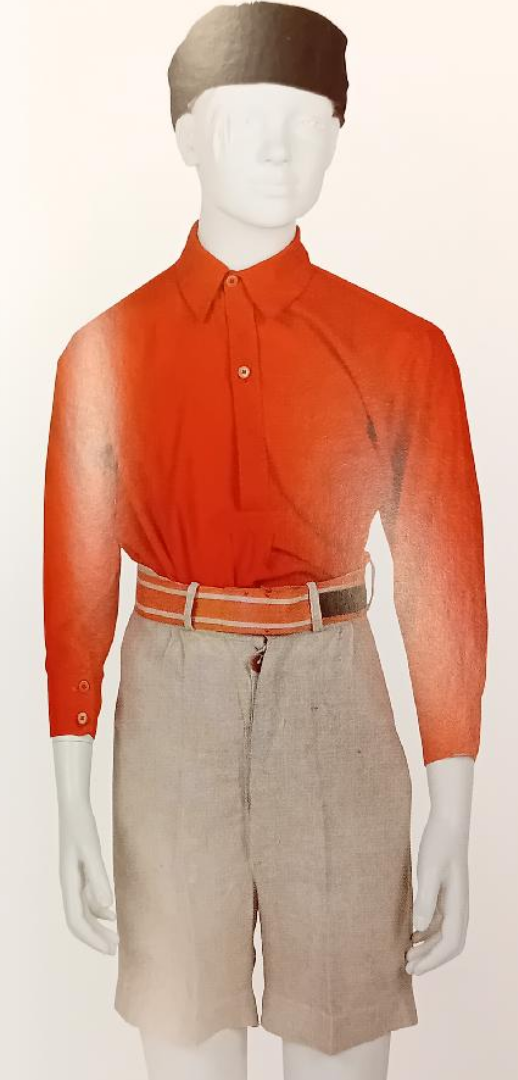
\includegraphics[width=0.98\linewidth]{kroj_zak.png} 
\end{minipage}
\begin{minipage}{0.6\linewidth}
  \center
  \textbf{Kroj žáci} – pro chlapce 6–15 let

  \begin{itemize}[itemsep=-3pt,leftmargin=2em]
    \item červená košile s~dlouhým rukávem (obyčejná koupená)
    \item šortky nad kolena z~režného plátna s~poutky na pásek (do gumy nebo na zip)
    \item černá čapka \luv{}hrnec\ruv{} s~červeným středem
    \item pásek – červený široký 4–5\,cm, se dvěma bílými pruhy
    \item tmavé boty a černé vysoké ponožky / podkolenky
  \end{itemize}
\end{minipage}

\vspace*{24pt}

\begin{minipage}{0.6\linewidth}
  \center
  \textbf{Kroj dorostenci} – pro chlapce 15–18 let

  \begin{itemize}[itemsep=-3pt,leftmargin=2em]
    \item bílá košile s~dlouhým rukávem (obyčejná koupená)
    \item bílé kalhoty ke kolenům s~třásněmi na spodním okraji
    \item sokolská čapka
    \item opasek \luv{}dohoda\ruv{} (v~antikvariátu nebo v~armyshopu)
    \item černé boty a podkolenky
  \end{itemize}
\end{minipage}
\begin{minipage}{0.3\linewidth}
  \hspace*{1em}
  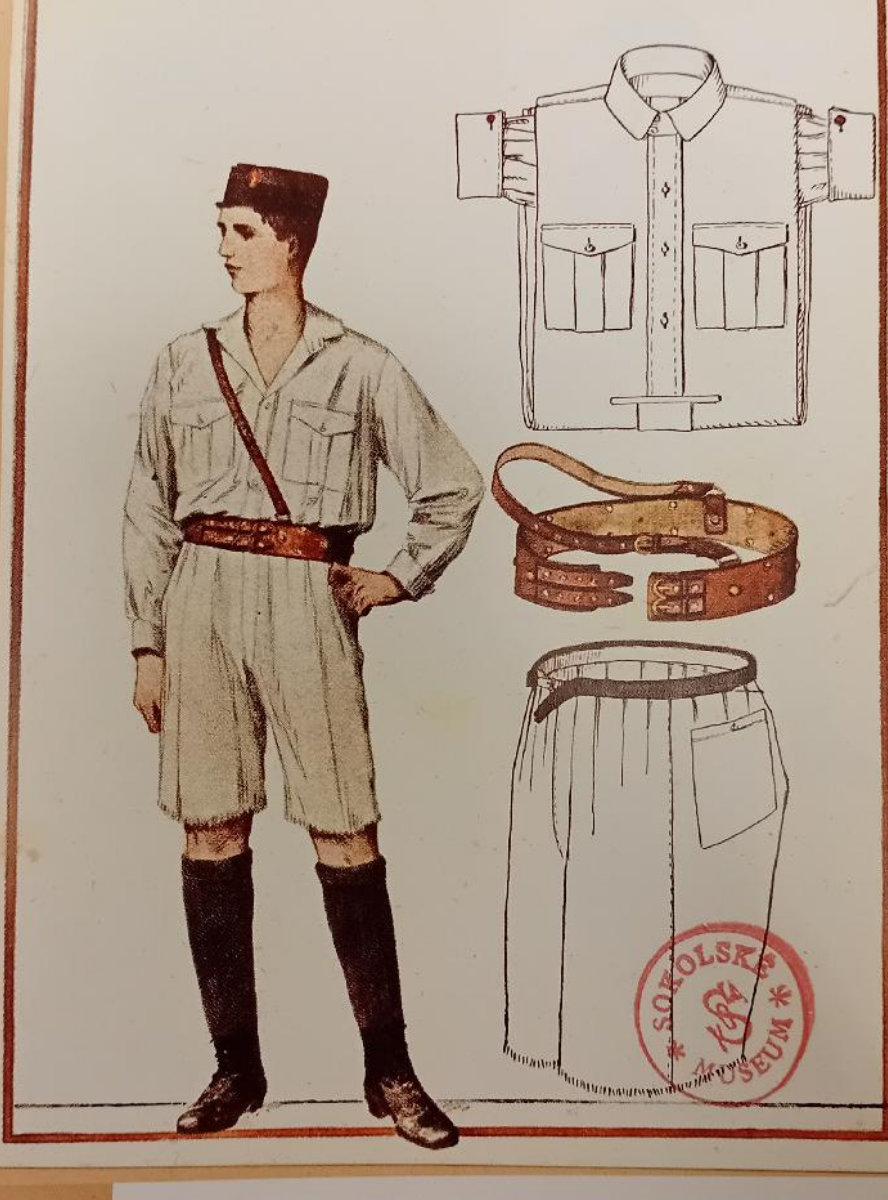
\includegraphics[width=0.98\linewidth]{kroj_dorostenec.png} 
\end{minipage}

\begin{minipage}{0.3\linewidth}   
  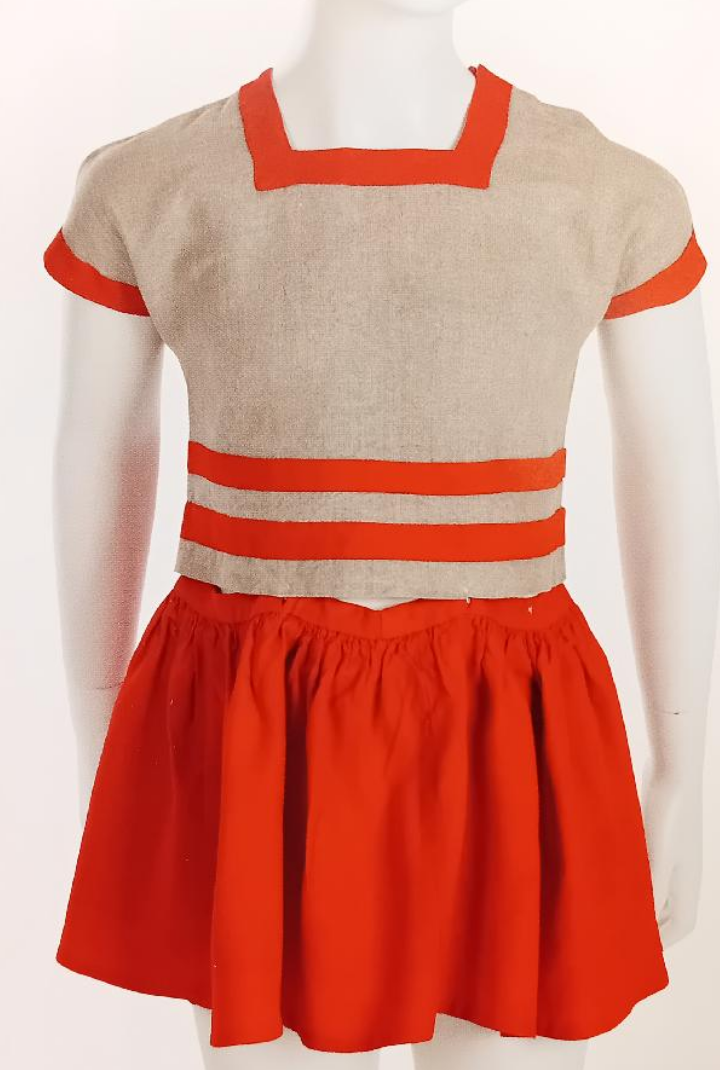
\includegraphics[width=0.98\linewidth]{kroj_zakyne.png} 
\end{minipage}
\begin{minipage}{0.6\linewidth}
  \center
  \textbf{Kroj žákyně mladší} – dívky 6–10 let

  \begin{itemize}[itemsep=-3pt,leftmargin=2em]
    \item režná halenka s~červenými pruhy
    \item červená nabíraná sukně, připojená knoflíky/patenty k~halence
    \item bílé nebo černé \luv{}boty k~sukni\ruv{}, silonky nebo nízké bílé nebo černé ponožky
  \end{itemize}
\end{minipage}

\vspace*{24pt}

\begin{minipage}{0.6\linewidth}
  \center
  \textbf{Kroj žákyně starší} – dívky 10–15 let
  
  \begin{itemize}[itemsep=-3pt,leftmargin=2em]
    \item modré šaty rovného střihu se sámky na ramenou, vyšívané šedou šujtaškou
    \item šedá kroucená šňůra coby pásek
    \item bílé nebo černé \luv{}boty k~sukni\ruv{}, silonky nebo nízké bílé nebo černé ponožky
  \end{itemize}
\end{minipage}
\begin{minipage}{0.3\linewidth}
  \hspace*{1em}
  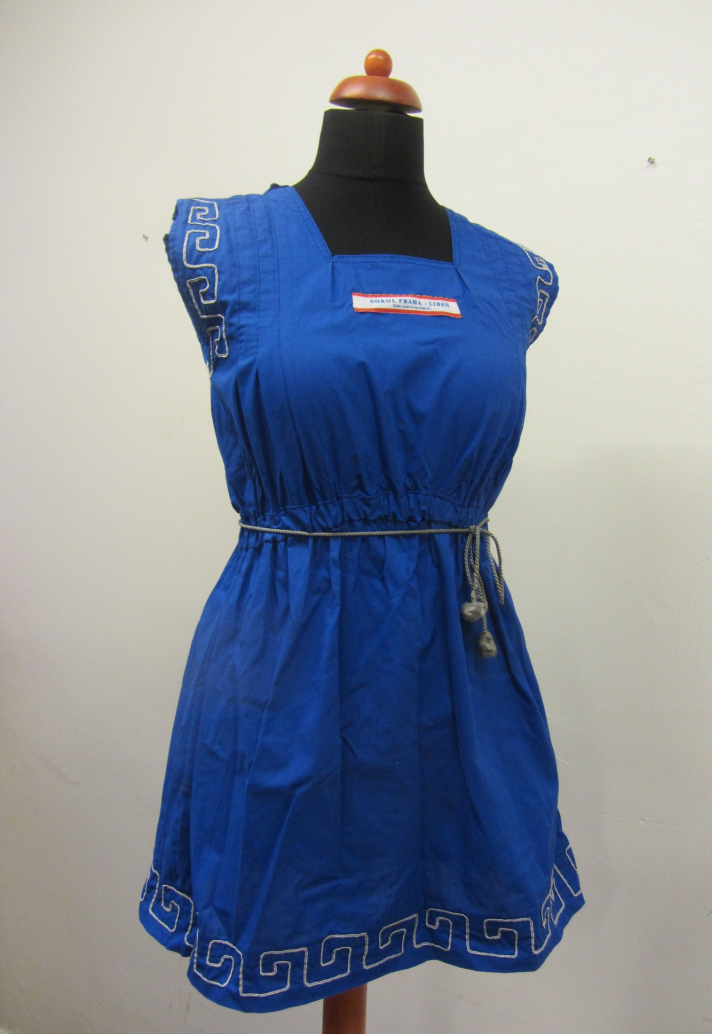
\includegraphics[width=0.98\linewidth]{kroj_st_zakyne.png} 
\end{minipage}

\vspace*{24pt}

\begin{minipage}{0.3\linewidth}   
  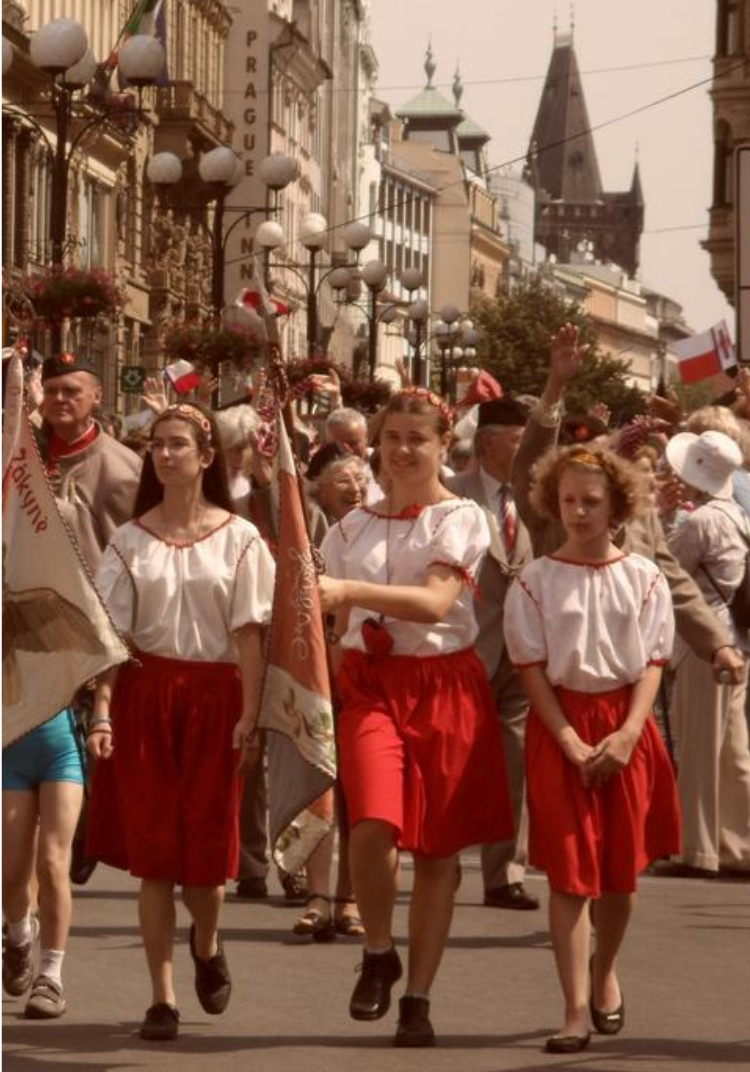
\includegraphics[width=0.98\linewidth]{kroj_dorostenka.png} 
\end{minipage}
\begin{minipage}{0.6\linewidth}
  \center
  \textbf{Kroj dorostenky} – dívky 15–18 let

  \begin{itemize}[itemsep=-3pt,leftmargin=2em]
    \item bílá halenka raglánového střihu s~širokými rukávy, olemovaná výšivkou, skrz kterou je protažená stužka a rukávy stažené \luv{}do balonku\ruv{}
    \item červená čtvrtkolová sukně ke kolenům
    \item červená čelenka s~našitými filcovými květy
    \item bílé nebo černé \luv{}boty k~sukni\ruv{}, silonky nebo nízké bílé nebo černé ponožky
  \end{itemize}
\end{minipage}

\signature{Anka Holanová}{}

\post{Pozvánka na loutkové divadlo}
Náš divadelní soubor Nástup pro vás v~sokolovně připravil v~prosinci následující divadelní představení:

\textbf{21. prosince 2023 (čt) od 17:00 ve Strnadově sále sokolovny: Vánoční Sokol}

Jde o~reprízu našeho loňského představení, se kterým se nám podařilo probojovat až na Loutkářskou Chrudim. Naše trojice malých sokolíků se na Vánoce nedopatřením ocitne zamčená v~naší sokolovně a při té příležitosti zažijí nemalé dobrodružství a nakonec i vánoční zázrak. Ti z~našich diváků, kteří by čekání již nemohli vydržet, budou moci toto představení shlédnout v~předstihu již 16. prosince 2023 (so) od 17:00 v~pobočce Městské knihovny v~Löwitově mlýně.  

\signature{Tomáš Troup}{principál}
\vspace*{12pt}
\noindent
\includegraphics*[width=\linewidth]{Vanocni_Sokol_sal_21_12_2023.png}

\clearpage



% zadní strana

\clearpage
\pagestyle{blank}
\newgeometry{margin=1cm}

\vspace*{96pt}

\pagecolor{sokolred}
\color{white}

\noindent {\fontsize{48pt}{56pt}\tyrs
se sokolským

\vspace*{24pt}

\noindent nazdar!}

\vspace*{\fill}

% \color{black}
\begin{center}
Vydává Tělocvičná jednota Sokol Libeň, Zenklova 37, Praha 8

\vspace*{12pt}

Na přípravě tohoto čísla se spolu s~autory jednotlivých textů podíleli:

grafická úprava – Martin Burian | jazyková úprava – Martina Waclawičová \\ editoři textů – Vít Jakoubek, Jan Přech
\end{center}

\end{document}